\section{RabbitMQ}

\subsection{Présentation générale}

RabbitMQ est un middleware de Pivotal facilitant l’échange de messages entre applications présentes sur un système informatique :  message broker software. RabbitMQ implémente le protocole AMQP (conçu par un consortium international) qui standardise les échanges de messages. Écrit en Erlang, RabbitMQ est open-source et un support payant est disponible. Des librairies sont disponibles pour l’écrasante majorité des langages utilisés, est compatible avec les principaux systèmes d’exploitation et bénéficie d’une large communauté d’utilisateurs. Il est utilisé par de nombreuses entreprises pour répondre à leurs besoins en échange de messages, telles que Instagram, The New York Times, Nokia, SoundCloud...

\subsection{Fonctionnalités}

RabbitMQ propose les fonctionnalités suivantes :

\begin{itemize}
  \item Le transport de messages ;
  \item La communication asynchrone : L’émetteur d'un message et le récepteur du message n'ont pas besoin d'être activés en même temps. La file d’attente reçoit le message de l'application émettrice et le stocke jusqu'à ce que l'application réceptrice vienne lire le message ;
  \item Le routage : Les messages peuvent être routés entre machines ;
  \item Le clustering : Plusieurs serveurs RabbitMQ peuvent former un cluster ;
  \item La persistance des messages : Les messages d’une file peuvent être sauvegardé sur un support physique ;
  \item La fiabilité : Chaque envoi ou réception par une application fait l'objet d'un accusé de réception. Couplé avec la persistance, ce mécanisme permet de garantir qu'aucun message ne sera perdu dans son transfert entre les applications ;
  \item La diversité des protocoles supportés : AMQP, STOMP, MQTT, AMQP, HTTP ;
  \item La diversité des clients : Java, Python, .NET, Ruby, PHP, etc… (plus de 20).
\end{itemize}

\subsection{Principes de fonctionnement}

RabbitMQ propose les différents cas d'utilisation :
\begin{itemize}
	\item Point à point : Une seule application productrice et une seule consommatrice. Le message est retiré de la file d’attente lorsque le consommateur l’a lu ;
	\item Publish-subscribe : Les applications consommatrices des messages s'abonnent à un channel correspondant à une catégorie de messages qu’elles veulent recevoir. Tous les messages du channel restent disponibles tant que tous les abonnés ne les ont pas lu ;
	\item Work queue : Une application remplit une file de job à exécuter. Des serveurs viennent récupérer ces tâches pour les réaliser.
	\item Routing : Les messages sont distribués dans les queues en fonction de leur type.
\end{itemize}
\ \\
La compréhension de RabbitMQ se limite à deux concepts :
\begin{itemize}
	\item la queue : c'est une file virtuelle de type FIFO dans laquelle des clients vont venir déposer ou récupérer des messages.
	\item l'exchange : c'est une sorte de routeur qu'un émetteur va créer et dans lequel il va déposer des messages. Sa fonction de routeur réside dans le fait que l'on peut configurer la manière dont il va diffuser les messages. Par exemple, je fais suivre tout les messages de type "error" dans toutes les queues dont le nom correspond au partern "*error*".
\end{itemize}
Dans les faits, les émetteurs créent des exchanges dans lesquelles ils publient des messages. Les récepteurs eux, viennent brancher des queues aux exchanges pour récupérer les messages.

\subsection{Infrastructure mise en place}

\begin{figure}
    \centering
    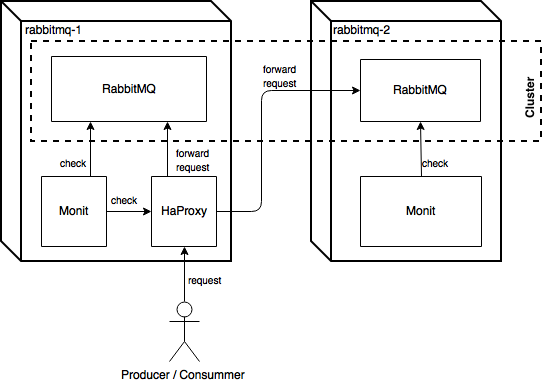
\includegraphics[scale=0.5]{pics/rabbitmq-infra.png}
    \caption{Schéma global de l'infrastructure mise en place pour RabbitMQ}
\end{figure}
\FloatBarrier
\subsubsection{Haute disponibilité}

Pour se prémunir d'une éventuelle panne d'un serveur et pour garantir une disponibilité du service, RabbitMQ propose un système de cluster. Dans notre application deux serveurs RabbitMQ forment un cluster. La réplication des queues de message peut être configurée. Dans notre cas nous avons fait le choix du répliquer par défaut toutes les queues présentes.

\subsubsection{Sécurité}

L'accès au service de RabbitMQ est sécurisé par des crédentials. Deux utilisateurs existent : spark\_user et neo4j\_user. Les services souhaitant publier des messages au sein du cluster doivent obligatoirement être authentifié auprès de ce dernier. Dans le cas contraire, la requête est rejetée. Là encore les droits applicable sur les utilisateurs peuvent être configurés (droit en lecture, droit en écriture, type de queue, espace virtuel, etc...). Dans notre application nous n'avons pas configuré de droit spécifique car un isolement plus fin n'était pas pertinent.

\subsubsection{Répartition de charge / DNS}

Malgré la présence d'un cluster RabbitMQ, un client qui souhaite poster/récupérer un message doit quand même spécifier le serveur sur lequel il doit se connecter. Pour supprimer au sein des clients l'intelligence de se connecter sur un serveur A ou B suivant les machines disponibles, nous avons mis en place un load balancer, ici HaProxy. Ce dernier à la responsabilité de rediriger et répartir les requêtes en fonction des machines disponibles qu'il connait. Ainsi, les clients ne se posent plus de questions. Ils n'ont à connaître qu'une seule adresse/port. Bien sûr ce choix technique est critiquable. En effet, si la machine qui héberge le load balancer tombe nous aurons une indisponibilité de service. Mais c'est un choix que nous avons fait pour décharger les clients de la problématique décrite plus haut.

\subsubsection{Monitoring}

Sur les deux machines rabbitmq-1 et rabbitmq-2 un Monit est installé. Il surveille l'état de certains services et est capable, lorsqu'il le détecte, de redémarrer les services qui seraient potentiellement hors service. La configuration de la surveillance est la suivante :
\begin{itemize}
	\item rabbitmq-1 : rabbitmq-server et haproxy ;
	\item rabbitmq-2 : rabbitmq-server.
\end{itemize}
\ \\
De plus, une interface de management est disponible. Elle permet de voir plusieurs paramètres concernant le cluster:
\begin{itemize}
	\item état du cluster ;
	\item queue/exhange en cours ;
	\item connections en cours ;
	\item activité en lecture et écriture ;
	\item poster/lire des messages ;
	\item etc ...
\end{itemize}

Cette interface web est disponible via l'url \textit{http://[rabbitmq-1|rabbitmq-2]:15672}

\subsubsection{Déploiement}

Le déploiement des serveurs, du HaProxy et du Monit est totalement automatisé et est assuré par des scripts python. Le déroulement de cette phase est la suivante :
\ \\
\begin{figure}[h]
    \centering
    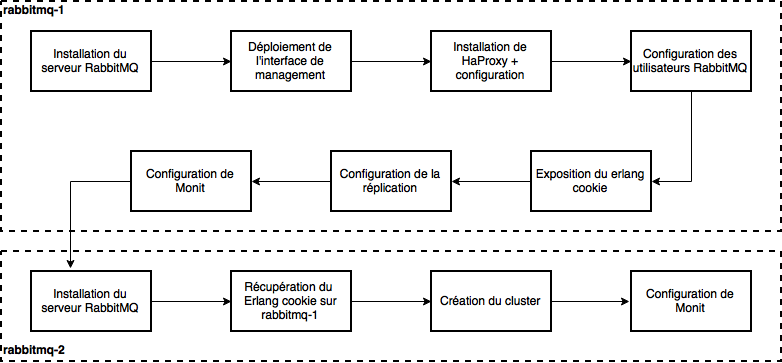
\includegraphics[scale=0.4]{pics/rabbitmq_deploy.png}
    \caption{Fluxs de la procédure de déploiement de RabbitMQ}
\end{figure}
\ \\
Remarques:
\begin{itemize}
	\item La récupération du Erlang cookie de rabbitmq-1 par rabbitmq-2 est une condition nécessaire pour permettre la formation du cluster.
	\item La configuration des utilisateurs et des paramètres de réplication n'est obligatoire que sur un serveur. En effet, lors de la création du cluster ils se synchronisent.
\end{itemize}

\subsubsection{Rôle applicatif}

Dans notre application, RabbitMQ fait le lien entre les demandes de recommandation pour un utilisateur faites par Mazerunner API et le calcul de la recommandation calculer par orchestrator/jobSpark. Il y a donc 2 exchanges et 2 queues (jobs\_to\_do et jobs\_done). Ils ont la respectivement la responsibilité de faire suivre les noms d'utilisateurs pour lesquels les recommandations sont à calculer, et ceux pour lesquels le calcul est terminé. Le schéma suivant résume son rôle:
\ \\
\begin{figure}[h]
    \centering
    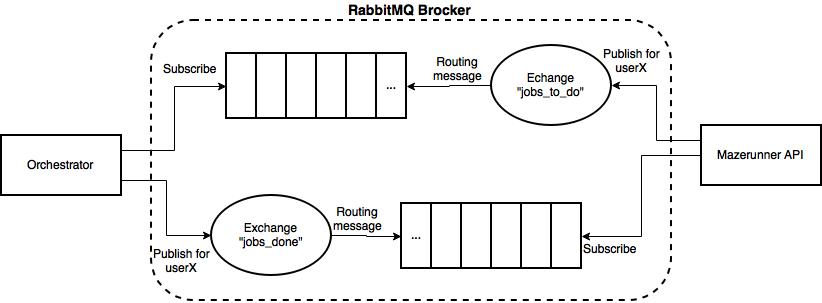
\includegraphics[scale=0.4]{pics/rabbitmq_role.png}
    \caption{Schéma synthétique illustrant le rôle applicatif de RabbitMQ}
\end{figure}
\FloatBarrier
